\subsubsection{Objective}
The third research question investigates how the installation dates and operational periods of weather stations affect data availability over time and across Austrian regions and elevation zones. The goal is to identify spatial and temporal coverage gaps, also referred to as ``data deserts,'' that could affect the interpretation of long-term climate analyses.

\subsubsection{Methodology}

To address this question, the implementation proceeded in two main steps:

\begin{enumerate}
  \item \textbf{Metadata-Based Coverage Matrix:}  
    Using station metadata (installation and deactivation dates), a year-by-year activity matrix was constructed from 1960 to 2025 using a cross join. Active periods were filtered, and each station was assigned to one of five elevation bands (same of RQ1).
    Aggregated counts by year, elevation zone, and federal state provided a theoretical view of station coverage.

  \item \textbf{Real Measurement-Based Coverage:}  
    To verify actual data presence, the climate dataset was filtered to include only records with at least one valid measurement. These were grouped using the same schema as the metadata-based approach.
\end{enumerate}

In this report, the results are shown for the Pre-Alps zone. The results for the other four zones can be found in the Jupyter Notebook.

\subsubsection{Results and Interpretation}

\paragraph{Figure~\ref{fig:coverage_meta_loweralps}: Metadata-Based Coverage (Lower Alps)}  
The heat map shows that Carinthia, Salzburg and Styria have maintained a consistent network of 7 to 16 active stations per year since the 1970s, while regions such as Lower Austria and Upper Austria are virtually absent or only sporadically represented in this altitude zone. While Vorarlberg is only moderately represented from 2008 onwards, only Tyrol has a good to very well-developed network over the entire period.

\begin{figure}[ht]
  \centering
    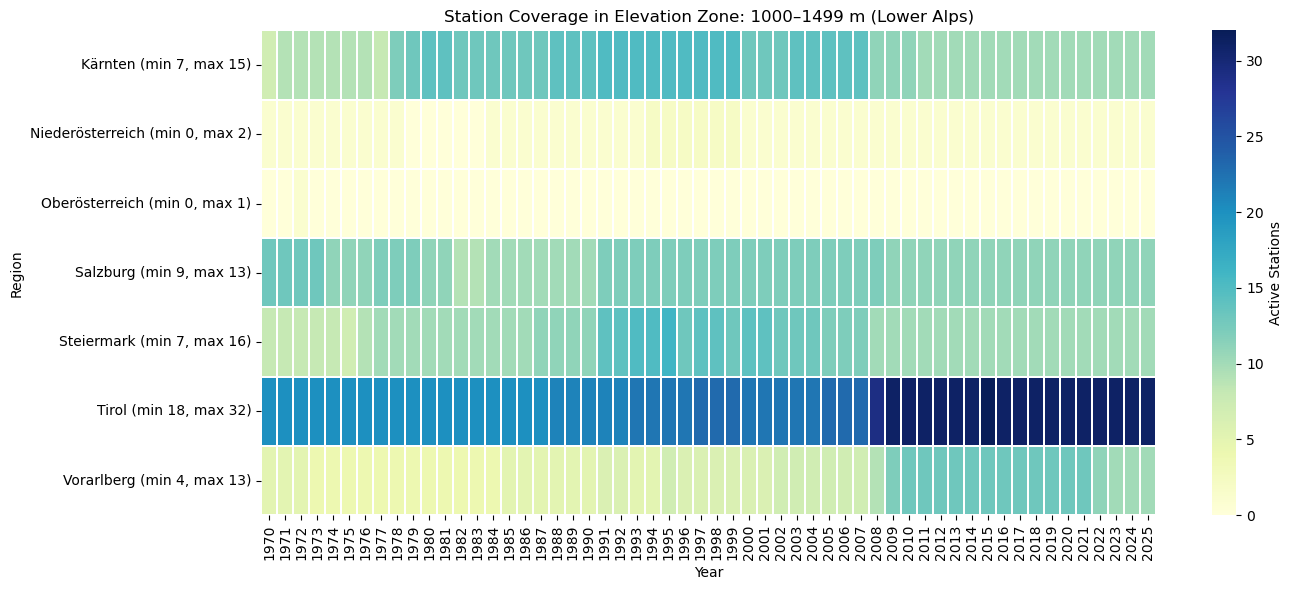
\includegraphics[width=0.45\textwidth]{img/coverage_zone_loweralps_meta.png}
    \caption{Metadata-based station coverage in elevation zone: 1000--1499\,m (Lower Alps)}
    \label{fig:coverage_meta_loweralps}
\end{figure}

\paragraph{Figure~\ref{fig:coverage_real_loweralps}: Actual Measurement-Based Coverage (Lower Alps)}  
The second heatmap confirms that actual measurement coverage aligns well with the metadata. Again, Tyrol is best represented, while several eastern federal states have minimal or no data-producing stations in this zone.

\begin{figure}[ht]
  \centering
    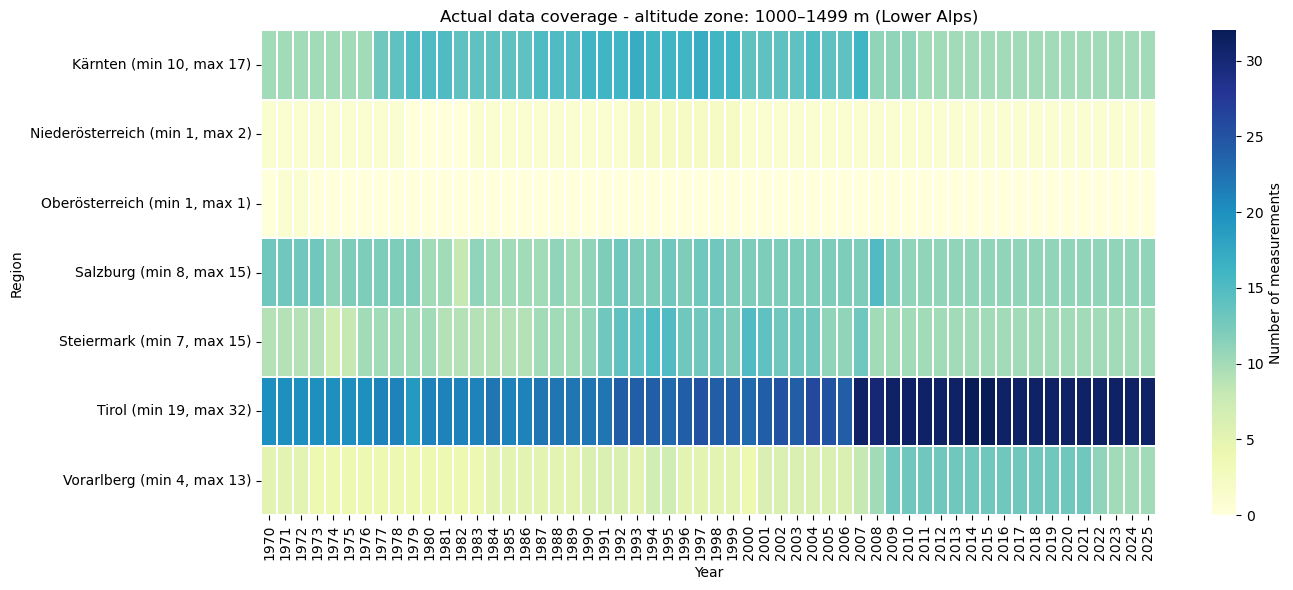
\includegraphics[width=0.45\textwidth]{img/data_coverage_loweralps.png}
    \caption{Actual measurement-based coverage in elevation zone: 1000--1499\,m (Lower Alps)}
    \label{fig:coverage_real_loweralps}
\end{figure}

\subsubsection{Conclusion}
Both the heat maps based on metadata and those based on actual measurements confirm consistent long-term detection gaps in the Lower Alps (1000-1499 m). This observation applies to several regions, especially in Upper and Lower Austria.

In the other altitude zones, too, the two representations of coverage agree well overall. However, there are slight differences in the shading (i.e. variations in the shades of blue) between the metadata and the measurement heat maps. These indicate periods in which the stations were technically active but provided little or incomplete data. A darker shade of blue in the measurement heatmaps compared to the same point in the metadata in turn indicates incorrect metadata or other data set errors.

It is therefore very important to validate assumptions based on metadata with the actual measurement results, especially for high-resolution or policy-relevant studies.
